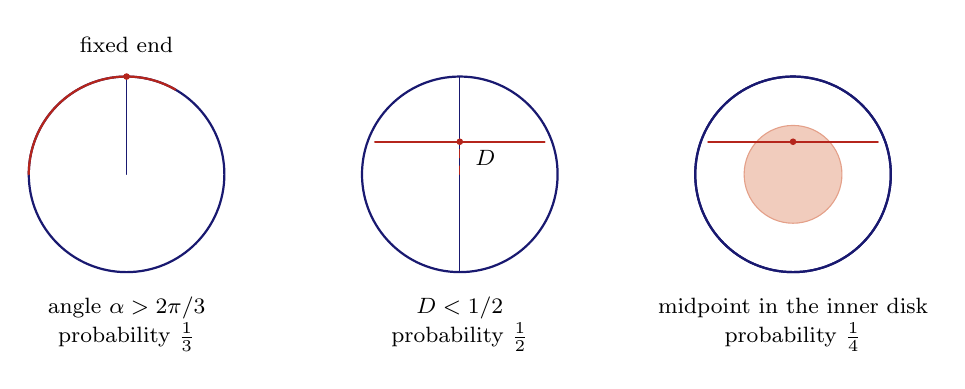
\begin{tikzpicture}[scale=0.92,line cap=round,line join=round]
  % Three models of a long chord. Radius 1.4.
  \begin{scope}
    \draw[MidnightBlue,thick] (0,0) circle (1.35);
    \draw[BrickRed,thick] (60:1.35) arc (60:180:1.35);
    \draw[MidnightBlue] (0,0) -- (90:1.35);
    \fill[BrickRed] (90:1.35) circle (1.3pt);
    \node[font=\footnotesize,anchor=south] at (90:1.55) {fixed end};
    \node[font=\footnotesize] at (0,-1.85) {angle $\alpha>2\pi/3$};
    \node[font=\footnotesize] at (0,-2.25) {probability $\frac13$};
  \end{scope}
  \begin{scope}[xshift=4.6cm]
    \draw[MidnightBlue,thick] (0,0) circle (1.35);
    \draw[MidnightBlue] (0,-1.35) -- (0,1.35);
    \draw[BrickRed,thick] (-1.17,0.45) -- (1.17,0.45);
    \fill[BrickRed] (0,0.45) circle (1.3pt);
    \draw[BrickRed,dashed] (0,0) -- (0,0.45);
    \node[font=\footnotesize,anchor=west] at (0.08,0.22) {$D$};
    \node[font=\footnotesize] at (0,-1.85) {$D<1/2$};
    \node[font=\footnotesize] at (0,-2.25) {probability $\frac12$};
  \end{scope}
  \begin{scope}[xshift=9.2cm]
    \draw[MidnightBlue,thick] (0,0) circle (1.35);
    \draw[BrickRed!35,fill=BrickRed!18] (0,0) circle (0.675);
    \draw[MidnightBlue,thick] (0,0) circle (1.35);
    \draw[BrickRed,thick] (-1.17,0.45) -- (1.17,0.45);
    \fill[BrickRed] (0,0.45) circle (1.3pt);
    \node[font=\footnotesize] at (0,-1.85) {midpoint in the inner disk};
    \node[font=\footnotesize] at (0,-2.25) {probability $\frac14$};
  \end{scope}
\end{tikzpicture}
